% =====================================================================
%  Oficina · XII Bienal da SBM · UFRN, Natal-RN · 3-7 de agosto de 2026
%  Autor: Pablo Nogueira Grossi (G6 LLC)
%  Tema: T2 — ajustar na submissão conforme o eixo temático selecionado
%  Título: A Escada de Recorrência — do k-nacci ao limiar τ = 2
% =====================================================================
\documentclass[11pt,a4paper]{article}

\usepackage[utf8]{inputenc}
\usepackage[T1]{fontenc}
\usepackage{lmodern}
\usepackage[a4paper,margin=2cm,top=2.8cm,bottom=2.2cm,headheight=18mm,headsep=6mm]{geometry}
% babel-portuguese não disponível neste TeX Live; forçamos rótulos manualmente:
\renewcommand{\tablename}{Tabela}
\renewcommand{\figurename}{Figura}
\usepackage{amsmath,amssymb,amsthm}
\usepackage{booktabs}
\usepackage{enumitem}
\usepackage{graphicx}
\usepackage{fancyhdr}
\usepackage[hidelinks]{hyperref}

% ─── Cabeçalho e rodapé institucionais (UFRN + XII Bienal SBM 2026) ──
\newcommand{\institutionalheader}{%
  \fancyhf{}%
  \fancyhead[L]{\raisebox{-0.35\height}{
\includegraphics[height=9mm]{assets/ufrn-logo.png}}}%
  \fancyhead[R]{\raisebox{-0.35\height}{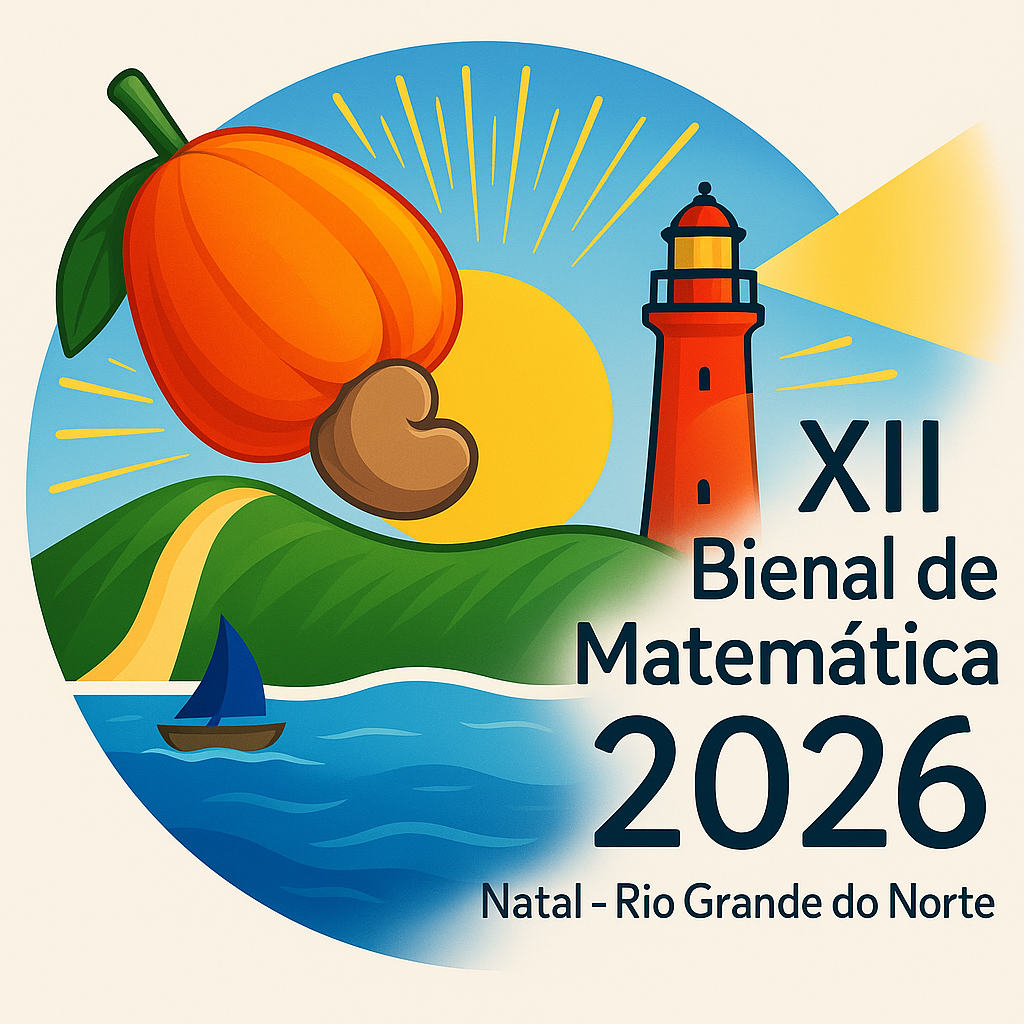
\includegraphics[height=13mm]{assets/bienal-2026-logo.png}}}%
  \fancyfoot[L]{\tiny\textcopyright\ 2026 Pablo N. Grossi / G6 LLC \textbullet\ CC BY 4.0 \textbullet\ XII Bienal da SBM 2026}%
  \fancyfoot[R]{\tiny \thepage}%
  \renewcommand{\headrulewidth}{0.3pt}%
  \renewcommand{\footrulewidth}{0.3pt}%
}
\pagestyle{fancy}\institutionalheader
\fancypagestyle{plain}{\institutionalheader}

% ─── Metadados do documento ──────────────────────────────────────────
\title{\textbf{Oficina: A Escada de Recorrência}\\[0.3em]
\large Do k-nacci ao limiar $\tau = 2$}
\author{Pablo Nogueira Grossi\\
\small G6 LLC\\
\small \texttt{brodananda@gmail.com}}
\date{Submissão à XII Bienal da SBM --- UFRN, Natal-RN --- 2026}

\setlength{\parskip}{0.4em}
\setlength{\parindent}{0pt}

\begin{document}

\maketitle

% =====================================================================
\section*{Modalidade e Duração}
\noindent
\textbf{Modalidade:} Oficina (atividade prática-coletiva).\quad
\textbf{Duração:} 2 horas, em um único encontro.\quad
\textbf{Público-alvo:} estudantes de graduação em Matemática (a partir do segundo período) e professores da educação básica interessados em conexões entre recorrências lineares, álgebra e dinâmica discreta.\quad
\textbf{Pré-requisitos:} cálculo diferencial de uma variável e noções de álgebra linear (autovalores de matrizes $2\times 2$).

% =====================================================================
\section*{Resumo}

Esta oficina propõe uma exploração hands-on de uma família de recorrências lineares que chamamos de \emph{k-nacci}: a generalização da sequência de Fibonacci em que cada termo é soma dos $k$ anteriores. Começando com $k=2$ (Fibonacci clássico, cuja razão áurea $\varphi \approx 1{,}618$ é a raiz dominante do polinômio característico $x^2 = x + 1$), os participantes, divididos em grupos, computam manualmente as raízes dominantes dos polinômios característicos para $k = 3, 4, 5, 6$ (Tribonacci, Tetranacci, Pentanacci, Hexanacci), e juntos constroem no quadro a \emph{Escada de Recorrência} $\pi \to \varphi \to \mu \to \eta \to \Delta \to \Sigma \to \Omega$, observando que a razão dominante $\tau_k$ converge monotonicamente para o valor limite $\tau = 2$ quando $k \to \infty$.

O objetivo central é triplo: (i) tornar tangível o conceito de polinômio característico de uma recorrência linear; (ii) oferecer uma experiência coletiva de descoberta matemática, em que cada grupo contribui com um degrau da escada e o padrão emerge apenas pela combinação das contribuições; e (iii) conectar um tema clássico de combinatória enumerativa (sequências de Fibonacci generalizadas) a uma ideia geométrica contemporânea ---  a de que $\tau = 2$ funciona como um \emph{limiar} na dinâmica de sistemas recorrentes, além do qual o comportamento qualitativo muda.

A oficina tem caráter experimental-didático: grupos pequenos (3 a 4 pessoas) recebem cada um um valor de $k$ e uma folha de trabalho; apresentam a raiz dominante obtida; a escada é construída coletivamente. O fechamento retoma o significado pedagógico de $\tau = 2$ como fronteira entre regimes dinâmicos ``subcríticos'' e ``supercríticos'', abrindo caminho para discussões em sistemas dinâmicos, modelagem biológica e dinâmica de populações.

% =====================================================================
\section*{Objetivos de Aprendizagem}

Ao final da oficina, espera-se que os participantes sejam capazes de:

\begin{enumerate}[leftmargin=2em,itemsep=0.2em]
  \item Formular o polinômio característico de uma recorrência linear de ordem $k$ da forma $a_{n} = a_{n-1} + a_{n-2} + \cdots + a_{n-k}$;
  \item Localizar numericamente (por bissecção ou método de Newton) a raiz dominante $\tau_k$ no intervalo $(1, 2)$;
  \item Reconhecer o padrão $\tau_k \nearrow 2$ e justificá-lo analiticamente por meio da observação de que $p_k(2) = 1$ para todo $k$;
  \item Discutir em grupo o significado qualitativo de $\tau = 2$ como limiar dinâmico, e relacionar a escada de recorrência a tópicos afins (sequências de Padovan, Lucas, problemas de pavimentação).
\end{enumerate}

% =====================================================================
\section*{A Escada de Recorrência --- Conteúdo Matemático}

Para cada inteiro $k \geq 2$, define-se a \emph{sequência k-nacci} $(a_n^{(k)})$ pela recorrência
\[
a_n^{(k)} = a_{n-1}^{(k)} + a_{n-2}^{(k)} + \cdots + a_{n-k}^{(k)},
\qquad \text{com condições iniciais apropriadas.}
\]
Sua equação característica é
\[
x^k = x^{k-1} + x^{k-2} + \cdots + x + 1,
\quad \text{ou equivalentemente} \quad
p_k(x) := x^{k+1} - 2x^{k} + 1 = 0.
\]
A raiz dominante $\tau_k \in (1, 2)$ --- única neste intervalo --- governa o crescimento assintótico da sequência: $a_n^{(k)} \sim C \cdot \tau_k^n$.

A Tabela~\ref{tab:escada} apresenta os sete primeiros degraus da escada, com nomenclatura grega adotada para expor a estrutura de saltos da escada (cada nome rotula uma posição específica no espectro).

\begin{table}[h]
\centering
\small
\begin{tabular}{@{}clcl@{}}
\toprule
Símbolo & Nome & $k$ & Raiz dominante $\tau_k$ \\
\midrule
$\pi$ & (basal, período) & --- & $1{,}000\,000\cdots$ (ponto fixo) \\
$\varphi$ & Fibonacci        & 2 & $1{,}618\,033\,988\cdots$ \\
$\mu$     & Tribonacci       & 3 & $1{,}839\,286\,755\cdots$ \\
$\eta$    & Tetranacci       & 4 & $1{,}927\,561\,975\cdots$ \\
$\Delta$  & Pentanacci       & 5 & $1{,}965\,948\,236\cdots$ \\
$\Sigma$  & Hexanacci        & 6 & $1{,}983\,582\,843\cdots$ \\
$\Omega$  & Heptanacci       & 7 & $1{,}991\,964\,197\cdots$ \\
$\tau$    & (limite)         & $\infty$ & $2{,}000\,000\,000\cdots$ \\
\bottomrule
\end{tabular}
\caption{A Escada de Recorrência --- sete degraus mais o limite.\label{tab:escada}}
\end{table}

O fato-chave --- a ser descoberto coletivamente na oficina --- é:
\[
\lim_{k \to \infty} \tau_k = 2,
\qquad\text{com a estimativa assintótica}\qquad
2 - \tau_k \sim \dfrac{1}{2^k}.
\]
A prova elementar combina duas observações: (i)~$p_k(2) = 2^{k+1} - 2^{k+1} + 1 = 1 > 0$, indicando que~$2$ nunca é raiz; (ii)~$p_k'(2) \to \infty$, de modo que a raiz ``aproxima-se de~$2$'' na taxa geométrica acima.

% =====================================================================
\section*{Metodologia Prática-Coletiva}

A oficina organiza-se em cinco blocos, totalizando 120 minutos.

\begin{table}[h]
\centering
\small
\begin{tabular}{@{}lp{0.65\linewidth}@{}}
\toprule
\textbf{Tempo} & \textbf{Atividade} \\
\midrule
0--15 min   & Introdução. Revisão rápida da recorrência de Fibonacci, demonstração da solução geral via polinômio característico, motivação da pergunta: \emph{o que acontece se somarmos mais termos?} \\
15--45 min  & Trabalho em grupos. Cada grupo recebe um $k \in \{3, 4, 5, 6, 7\}$ e folha de trabalho: (a)~escrever a recorrência; (b)~formar o polinômio característico; (c)~localizar $\tau_k$ por bissecção ou Newton (calculadora permitida). \\
45--75 min  & Apresentações. Cada grupo escreve no quadro o seu degrau $\tau_k$. O facilitador constrói a escada completa em tempo real, rotulando cada degrau com o símbolo grego correspondente. \\
75--100 min & Síntese matemática. Discussão coletiva: \emph{por que nenhum $\tau_k$ atinge~$2$?} Prova da identidade $p_k(2) = 1$. Observação empírica de que $2 - \tau_k$ decresce exponencialmente; justificativa heurística. \\
100--120 min & Extensões e conexões. Sequência de Padovan; pavimentações de domi\-nós; crescimento populacional em modelos de Leslie; menção à ocorrência de $\tau = 2$ como limiar em sistemas dinâmicos contínuos (ODE dissipativas, gastos energéticos em organismos). Encerramento: lista de leitura sugerida. \\
\bottomrule
\end{tabular}
\caption{Cronograma de 120 minutos, encontro único.}
\end{table}

\noindent\textbf{Materiais:} quadro-branco com espaço para a escada completa; calculadora ou celular; folhas A4 impressas com o roteiro (uma por grupo). Sem exigência de laboratório.

% =====================================================================
\section*{Relevância para os Eixos Temáticos da Bienal}

A oficina articula-se naturalmente com o eixo de \emph{Matemática e suas Aplicações}, por situar uma família clássica de recorrências em contato com ideias contemporâneas de dinâmica. Ao mesmo tempo, por seu formato acessível e coletivo, dialoga com o eixo de \emph{Formação de Professores} e com a \emph{Matemática na Educação Básica}, oferecendo a professores uma atividade replicável em sala de aula de ensino médio (com adaptações no grau de formalização da convergência).

% =====================================================================
\section*{Bibliografia}

\begin{enumerate}[leftmargin=2em,itemsep=0em]
  \item HOGGATT, V.~E. \emph{Fibonacci and Lucas Numbers}. Boston: Houghton Mifflin, 1969.
  \item GRAHAM, R.~L.; KNUTH, D.~E.; PATASHNIK, O. \emph{Concrete Mathematics}. 2.~ed. Addison-Wesley, 1994.
  \item KOSHY, T. \emph{Fibonacci and Lucas Numbers with Applications}. Wiley-Interscience, 2001.
  \item SLOANE, N.~J.~A. \emph{OEIS} --- sequências A000045, A000073, A000078, A001591, A001592. \url{https://oeis.org}.
  \item GROSSI, P.~N. Helical Attractors on Contact 3-Manifolds. In: \emph{Principia Orthogona}, Vol.~IV. G6 LLC, 2026. \url{https://totogt.github.io/3M/}.
\end{enumerate}

\vspace{1em}
\noindent\rule{\linewidth}{0.3pt}\\[0.3em]
\footnotesize
\emph{Submissão à XII Bienal da Sociedade Brasileira de Matemática. UFRN, Natal-RN, 3--7 de agosto de 2026. Categoria: Oficina (2h, encontro único). Código de tema: T2 (a confirmar no portal conforme eixo temático selecionado).}

\end{document}
